%%%%%%%%%%%%%%%%%%%%%%%%%%%%%%%%%%%%%%%%%%%%%%%%%%%%%%%%%%%%%%%%%%%%%%%%%%%%
% AGUJournalTemplate.tex: this template file is for articles formatted with LaTeX
%
% This file includes commands and instructions
% given in the order necessary to produce a final output that will
% satisfy AGU requirements, including customized APA reference formatting.
%
% You may copy this file and give it your
% article name, and enter your text.
%
%
% Step 1: Set the \documentclass
%
%

%% To submit your paper:
\documentclass[draft]{agujournal2019}
\usepackage{url} %this package should fix any errors with URLs in refs.
\usepackage{lineno}
\usepackage[inline]{trackchanges} %for better track changes. finalnew option will compile document with changes incorporated.
\usepackage{soul}
\linenumbers

%%%%%%%
% As of 2018 we recommend use of the TrackChanges package to mark revisions.
% The trackchanges package adds five new LaTeX commands:
%
%  \note[editor]{The note}
%  \annote[editor]{Text to annotate}{The note}
%  \add[editor]{Text to add}
%  \remove[editor]{Text to remove}
%  \change[editor]{Text to remove}{Text to add}
%
% complete documentation is here: http://trackchanges.sourceforge.net/
%%%%%%%

\draftfalse

%% Enter journal name below.
%% Choose from this list of Journals:
%
% JGR: Atmospheres
% JGR: Biogeosciences
% JGR: Earth Surface
% JGR: Oceans
% JGR: Planets
% JGR: Solid Earth
% JGR: Space Physics
% Global Biogeochemical Cycles
% Geophysical Research Letters
% Paleoceanography and Paleoclimatology
% Radio Science
% Reviews of Geophysics
% Tectonics
% Space Weather
% Water Resources Research
% Geochemistry, Geophysics, Geosystems
% Journal of Advances in Modeling Earth Systems (JAMES)
% Earth's Future
% Earth and Space Science
% Geohealth
%
% ie, \journalname{Water Resources Research}

\journalname{Journal of Advances in Modeling Earth Systems (JAMES)}


\begin{document}

%% ------------------------------------------------------------------------ %%
%  Title
%
% (A title should be specific, informative, and brief. Use
% abbreviations only if they are defined in the abstract. Titles that
% start with general keywords then specific terms are optimized in
% searches)
%
%% ------------------------------------------------------------------------ %%

% Example: \title{This is a test title}

\title{Impact of grids and dycores in CESM2.2 on the meteorology and climate of the Arctic}

%% ------------------------------------------------------------------------ %%
%
%  AUTHORS AND AFFILIATIONS
%
%% ------------------------------------------------------------------------ %%

% Authors are individuals who have significantly contributed to the
% research and preparation of the article. Group authors are allowed, if
% each author in the group is separately identified in an appendix.)

% List authors by first name or initial followed by last name and
% separated by commas. Use \affil{} to number affiliations, and
% \thanks{} for author notes.
% Additional author notes should be indicated with \thanks{} (for
% example, for current addresses).

% Example: \authors{A. B. Author\affil{1}\thanks{Current address, Antartica}, B. C. Author\affil{2,3}, and D. E.
% Author\affil{3,4}\thanks{Also funded by Monsanto.}}
\authors{Adam R. Herrington \affil{1}, Marcus Lofverstrom \affil{2}, Peter H. Lauritzen \affil{1} and Andrew Gettelman \affil{1}}

 \affiliation{1}{National Center for Atmospheric Research, 1850 Table Mesa Drive, Boulder, Colorado, USA}
\affiliation{2}{Department of Geosciences, University of Arizona, 1040 E. 4th Street, Tucson, AZ USA}

% \affiliation{1}{First Affiliation}
% \affiliation{2}{Second Affiliation}
% \affiliation{3}{Third Affiliation}
% \affiliation{4}{Fourth Affiliation}

%\affiliation{=number=}{=Affiliation Address=}
%(repeat as many times as is necessary)

%% Corresponding Author:
% Corresponding author mailing address and e-mail address:

% (include name and email addresses of the corresponding author.  More
% than one corresponding author is allowed in this LaTeX file and for
% publication; but only one corresponding author is allowed in our
% editorial system.)

% Example: \correspondingauthor{First and Last Name}{email@address.edu}

\correspondingauthor{=name=}{=email address=}

%% Keypoints, final entry on title page.

%  List up to three key points (at least one is required)
%  Key Points summarize the main points and conclusions of the article
%  Each must be 140 characters or fewer with no special characters or punctuation and must be complete sentences

% Example:
% \begin{keypoints}
% \item	List up to three key points (at least one is required)
% \item	Key Points summarize the main points and conclusions of the article
% \item	Each must be 140 characters or fewer with no special characters or punctuation and must be complete sentences
% \end{keypoints}

\begin{keypoints}
\item enter point 1 here
\item enter point 2 here
\item enter point 3 here
\end{keypoints}

%% ------------------------------------------------------------------------ %%
%
%  ABSTRACT and PLAIN LANGUAGE SUMMARY
%
% A good Abstract will begin with a short description of the problem
% being addressed, briefly describe the new data or analyses, then
% briefly states the main conclusion(s) and how they are supported and
% uncertainties.

% The Plain Language Summary should be written for a broad audience,
% including journalists and the science-interested public, that will not have 
% a background in your field.
%
% A Plain Language Summary is required in GRL, JGR: Planets, JGR: Biogeosciences,
% JGR: Oceans, G-Cubed, Reviews of Geophysics, and JAMES.
% see http://sharingscience.agu.org/creating-plain-language-summary/)
%
%% ------------------------------------------------------------------------ %%

%% \begin{abstract} starts the second page

\begin{abstract}
[ enter your Abstract here ]
\end{abstract}

\section*{Plain Language Summary}
[ enter your Plain Language Summary here or delete this section]


%% ------------------------------------------------------------------------ %%
%
%  TEXT
%
%% ------------------------------------------------------------------------ %%

%%% Suggested section heads:
\section{Introduction}

General Circulation Models (GCMs) are a powerful tool for understanding the meteorology and climate of the poles, which are among the most sensitive regions on Earth to global and environmental change. Despite their importance, numerically, not all GCMs treat the polar regions the same way as they do elsewhere in the domain due to the \textit{pole-problem} \cite{W2007JMSJ}. The wide variety of grids structures and numerical techniques used to represent polar regions in conventional GCMs are evaluated in this study for their impacts on the meteorology and climate of the Arctic.

The pole-problem refers to instability arising from the convergence of meridians into a polar singularity on latitude-longitude grids. In the 1970's this issue was largely defeated through wide-spread adaption of the spectral transform methods in GCMs, which transforms grid point fields into an isotropic representation in wave space. But as computing power has increased, local numerical methods have become more desirable for their ability to run efficiently on massively parallel systems. The pole-problem has thus re-emerged in contemporary climate models using latitude-longitude grids, and some combination of reduced grids and polar filters are necessary to subdue this instability \cite{JW2010LNCSE}. 

An alternative approach is to use unstructured grids. Unstructured grids permit quasi-uniform grid spacing globally, thereby eliminating the pole-problem. They allow for more flexible grid-structures than latitude-longitude grids, and can support regional grid refinement that may be used to capture higher resolution in the polar regions. Regional refinement of polar regions may be desirable as latitude-longitude grids, by virtue of the convergence of meridians, have higher horizontal resolution in polar regions compared to quasi-uniform grids containing the same degrees of freedom.

The meteorology and climate of the Arctic is charcterized by a range of processes and scales that are difficult to represent in GCMs \cite{BETAL2001MWR,SG2017MWR,VETAL2018TC}. The Arctic geography consists of a polar ocean surrounded by the northern coasts of the northern hemisphere continents and the large island of Greenland. Greenland is covered in a kilometers thick ice sheet, and receives a substantial portion of its snowfall from synoptic-scale storms traversing up the eastern sea-board of North America that rain out over its steep margins. Intense cold season Polar Lows traverse the Arctic's melange of sea-ice and open ocean, inducing gale-speed winds. Large volumes of fresh water drain into the ocean through river outlets in Canada and Russia, iceberg discharge and melt water runoff emanating from the margins of GrIS. As such, the Arctic serves as a test-bed for comparing the simulated meteorology and climate to different numerical treatments of polar regions.

The atmospheric component of the Community Earth System Model, version 2.2 (CESM; \url{http://www.cesm.ucar.edu/models/cesm2/}), the Community Atmosphere Model, version 6.3 (CAM; \url{https://github.com/ESCOMP/CAM/wiki}), supports a diverse number of atmospheric dynamical cores (hereafter referred to as \textit{dycores}). These range from dycores using latitude-longitude grids, the finite-volume \cite<FV;>{L2004MWR} and eulerian spectral transform \cite<EUL;>{CETAL006JC} models, and dycores built on unstructured grids, the spectral-element \cite<SE;>{LetAl2018JAMES} and finite-volume 3 \cite<FV3;>{PL2007JCP} models. The EUL dycore is the oldest dycore in CAM, and is the least supported of all the dycores. FV3 is the newest dycore in CESM, but it was not fully incorporated into the model at the time this work commenced, and so is omitted from this study. The authors instead focus on the two most well supported dycores in CESM, SE and FV. The goal of this study is to characterize the representation of polar regions using the SE and FV dycores, as these models treat the high-latitudes, e.g., the pole-problem, in very different ways. 

The FV dycore is assessed using grids with $\Delta x$ of $1^{\circ}$ and $2^{\circ}$ grid spacing ($\Delta x$ refers to the average equatorial grid spacing). These are compared to the equivalent  $1^{\circ}$ SE grid, referred to as ne30pg3. This grid does not refer to the SE dycore proper, but a variant in which the dry dynamics are solved using the SE method, and tracer advection computed using the conservative semi-Lagrangian advection method \cite <SE-CSLAM;>{LTOUNGK2017MWR}. In SE-CSLAM the physical parameterizations are computed on the finite-volume tracer advection grid. Optionally, one can compute the physics on a finite-volume grid that is $\frac{3}{2} \times \Delta x$ of the tracer-advection grid \cite{HETAL2019JAMES}. A comparison of the lower-resolution physics grid version of ne30pg3, referred to as ne30pg2, over the Arctic is included in this study. All variants of the SE dycore discussed herein are available as part of the CESM2.2 release.

The SE dycore (not SE-CSLAM) supports regional grid refinement via its variable resolution configuration. Two variable resolution meshes were developed as part of the CESM2.2 release that contains grid refinement over the Arctic. The ARCTIC grid is a $\Delta x=1^{\circ}$ grid with $\Delta x=\frac{1}{4}^{\circ}$ regional refinement over the broader Arctic region. The ARCTICGRIS grid is similar to the ARCTIC grid, but additionally contains a patch covering the big island of Greenland with $\Delta x=\frac{1}{8}^{\circ}$ resolution. These Arctic refined grids are depicted in Figure~\ref{fig:vr-grids}. The surface mass balance of the GrIS is compared across all grids and dycores in this study, and the ARCTCGRIS grid is certainly at an advantage due to its higher resolution over the ice sheet.

The study is laid out as follows. Section~\ref{sec:methods} consists of documentation of the grids, dycores and physical parameterizations used in this study. The Arctic refined grids were developed by the author, and this section serves as their official documentation. Section~\ref{sec:methods} also contains a description of the experiments along with the observational datasets and post-processing software used for validating the models. Section~\ref{sec:results} contains the results of the experiments and Section~\ref{sec:conclusions} provides some discussion and conclusions. 

\begin{figure}[t]
\begin{center}
\begin{tabular}{cccc}
         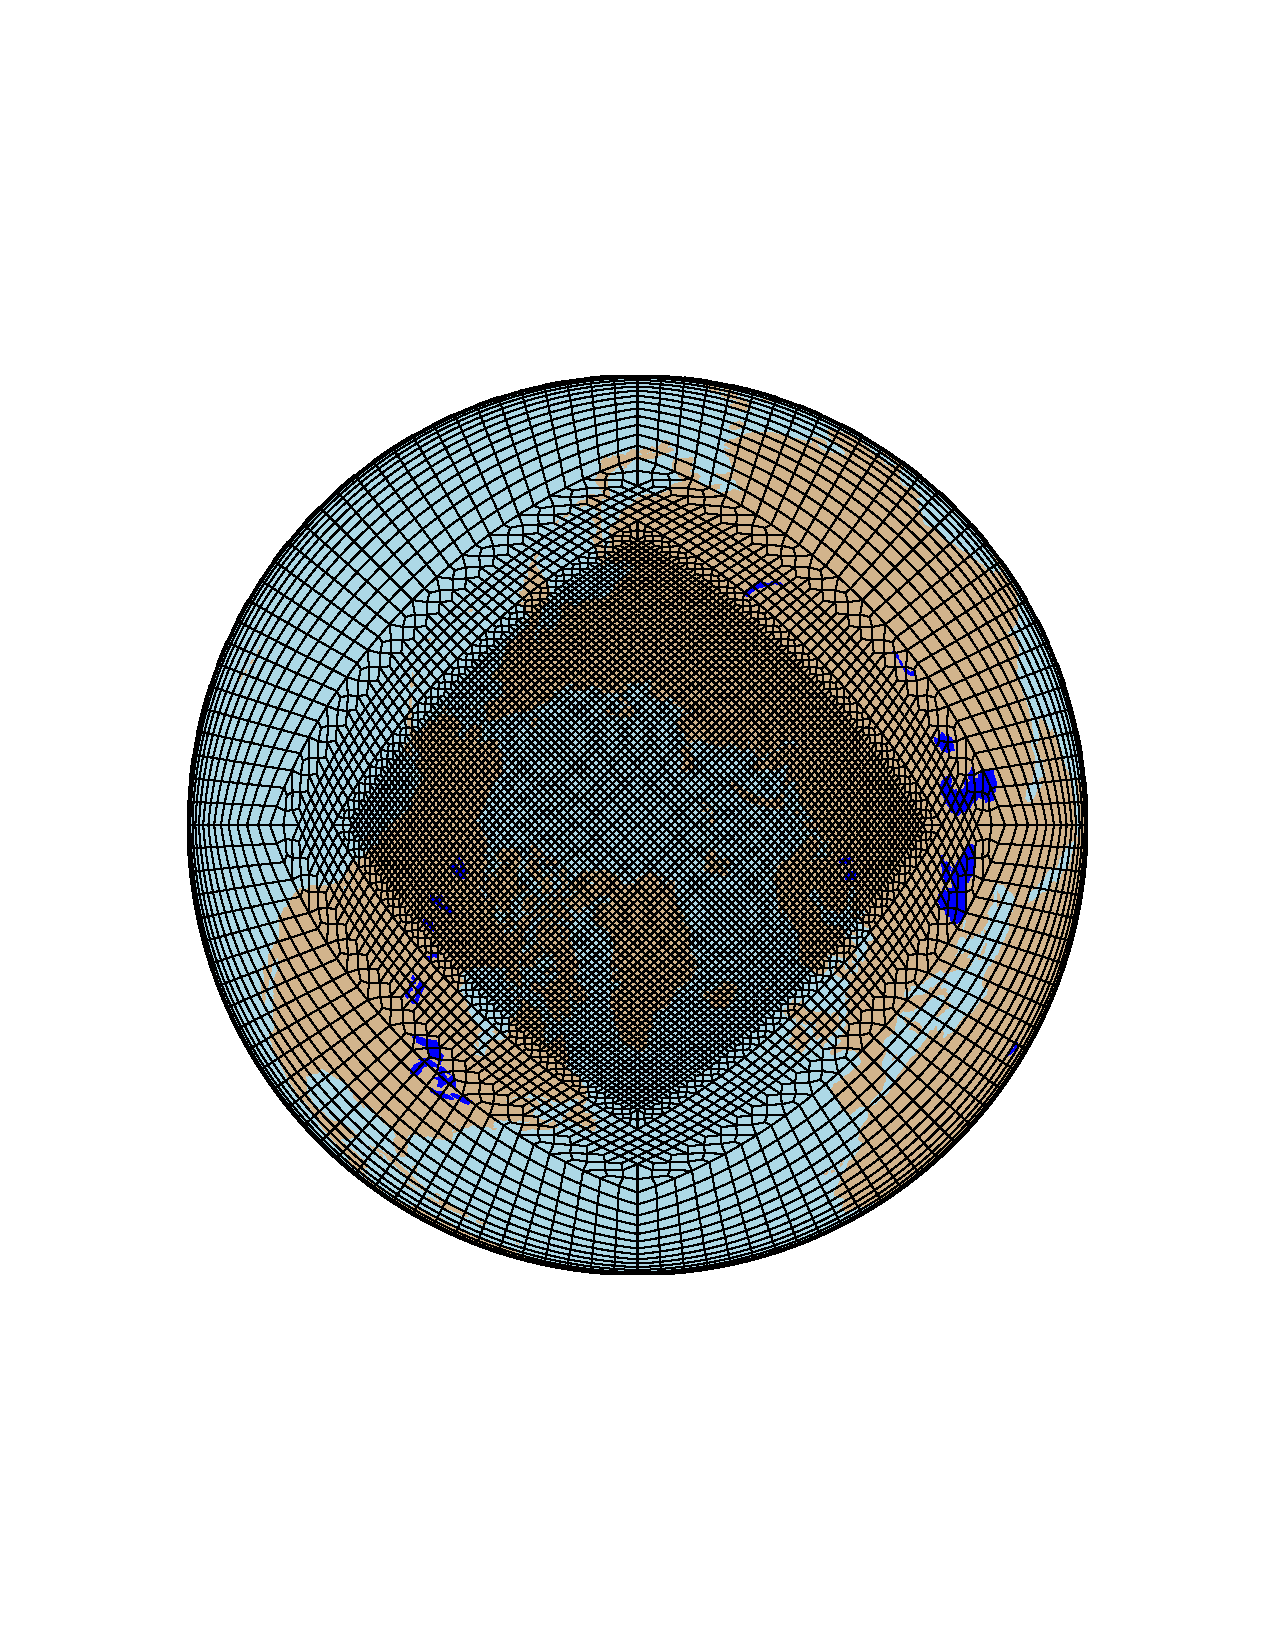
\includegraphics[width=60mm]{figs/grid-ARCTIC.pdf}&
         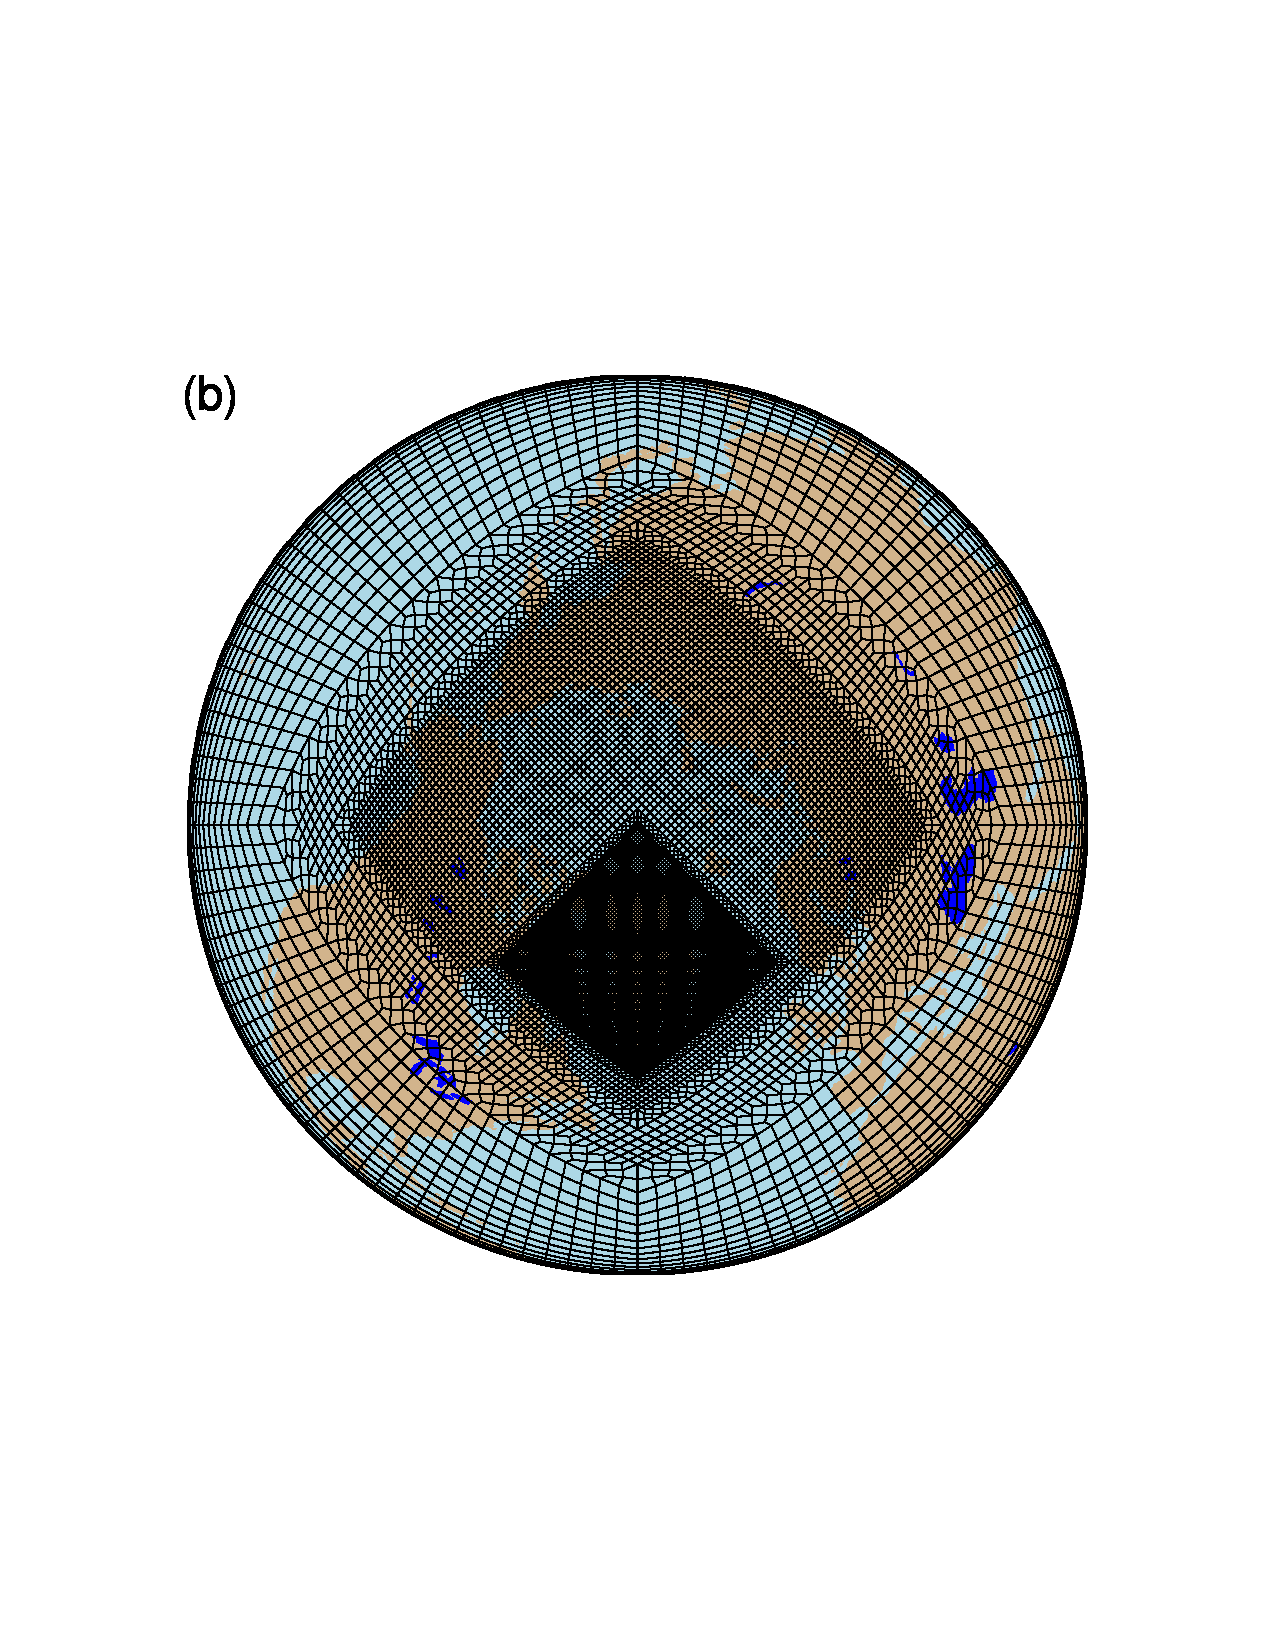
\includegraphics[width=60mm]{figs/grid-ARCTICGRIS.pdf} \\
\end{tabular}
\end{center}
\caption{.}
\label{fig:vr-grids}
\end{figure}

\begin{figure}[t]
\begin{center}
\begin{tabular}{cc}
         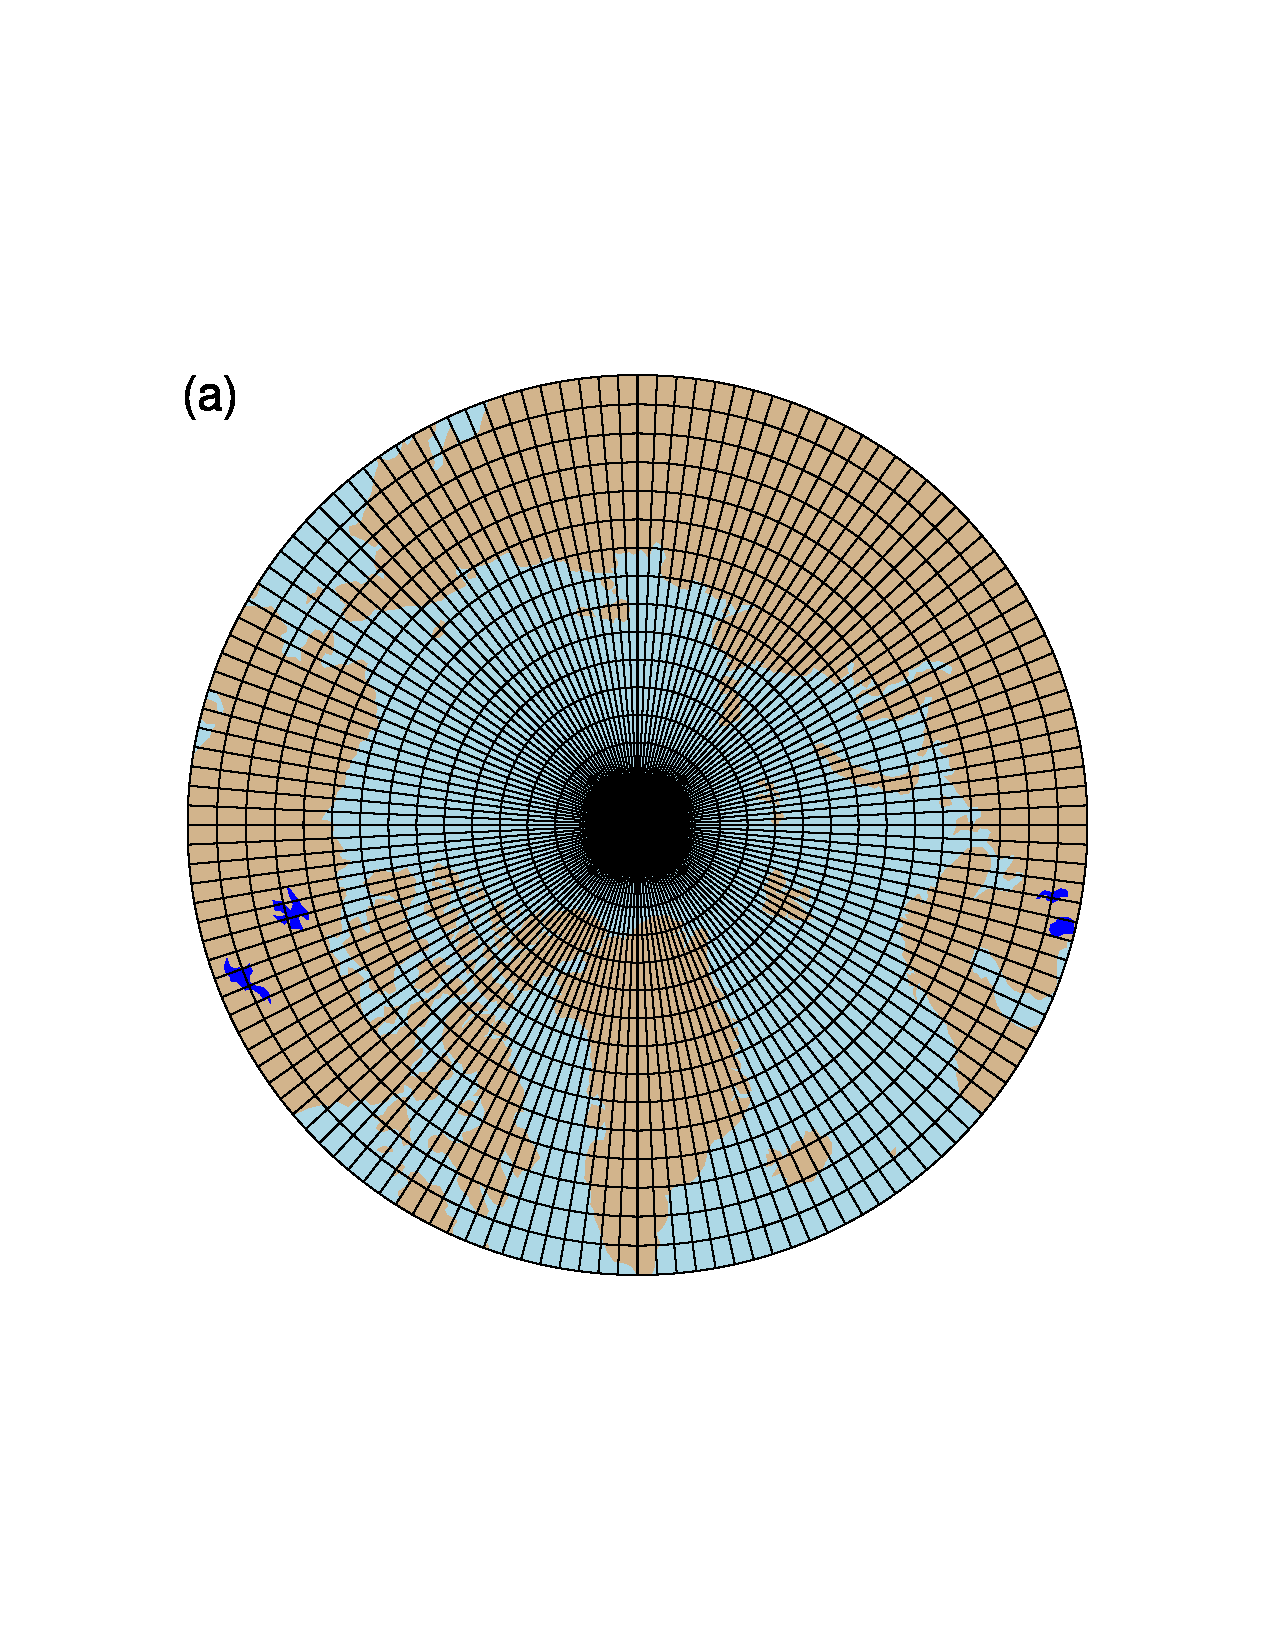
\includegraphics[width=60mm]{figs/grid-f19.pdf}&
         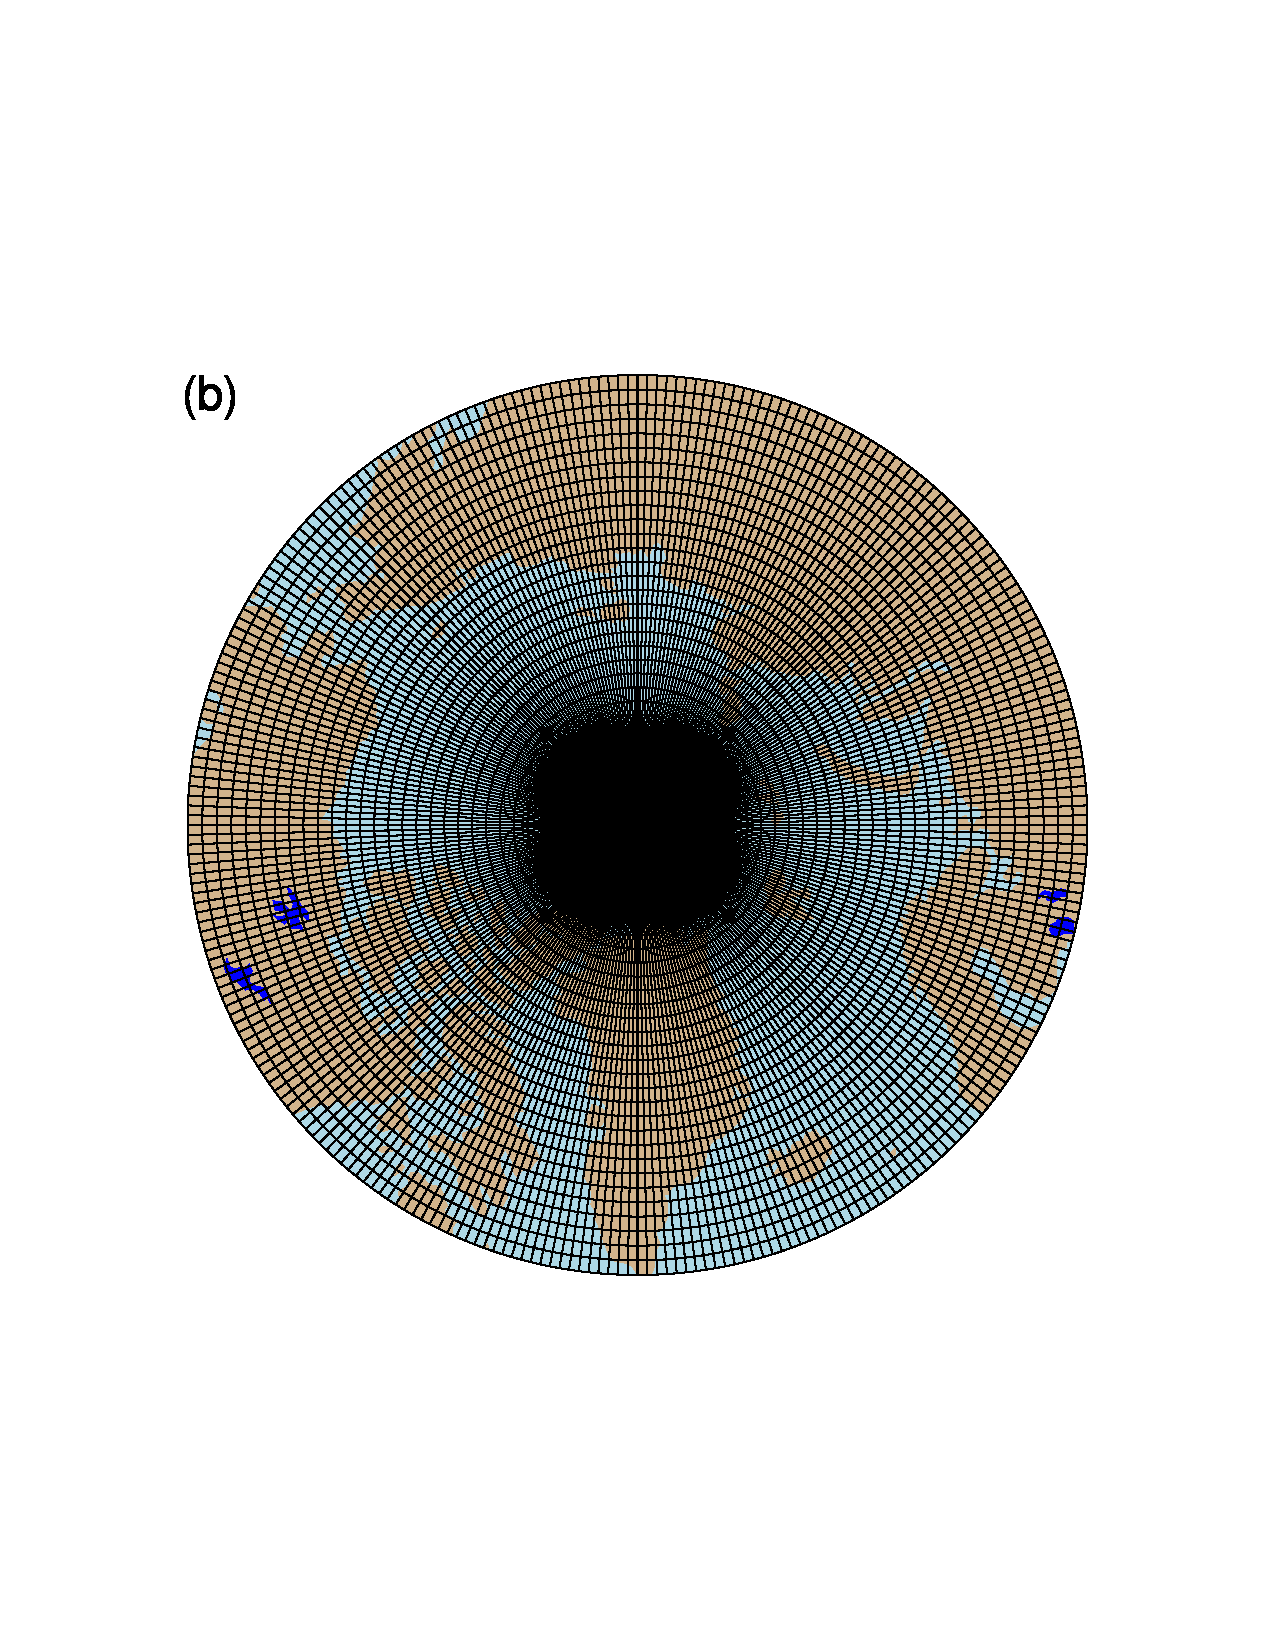
\includegraphics[width=60mm]{figs/grid-f09.pdf}\\
         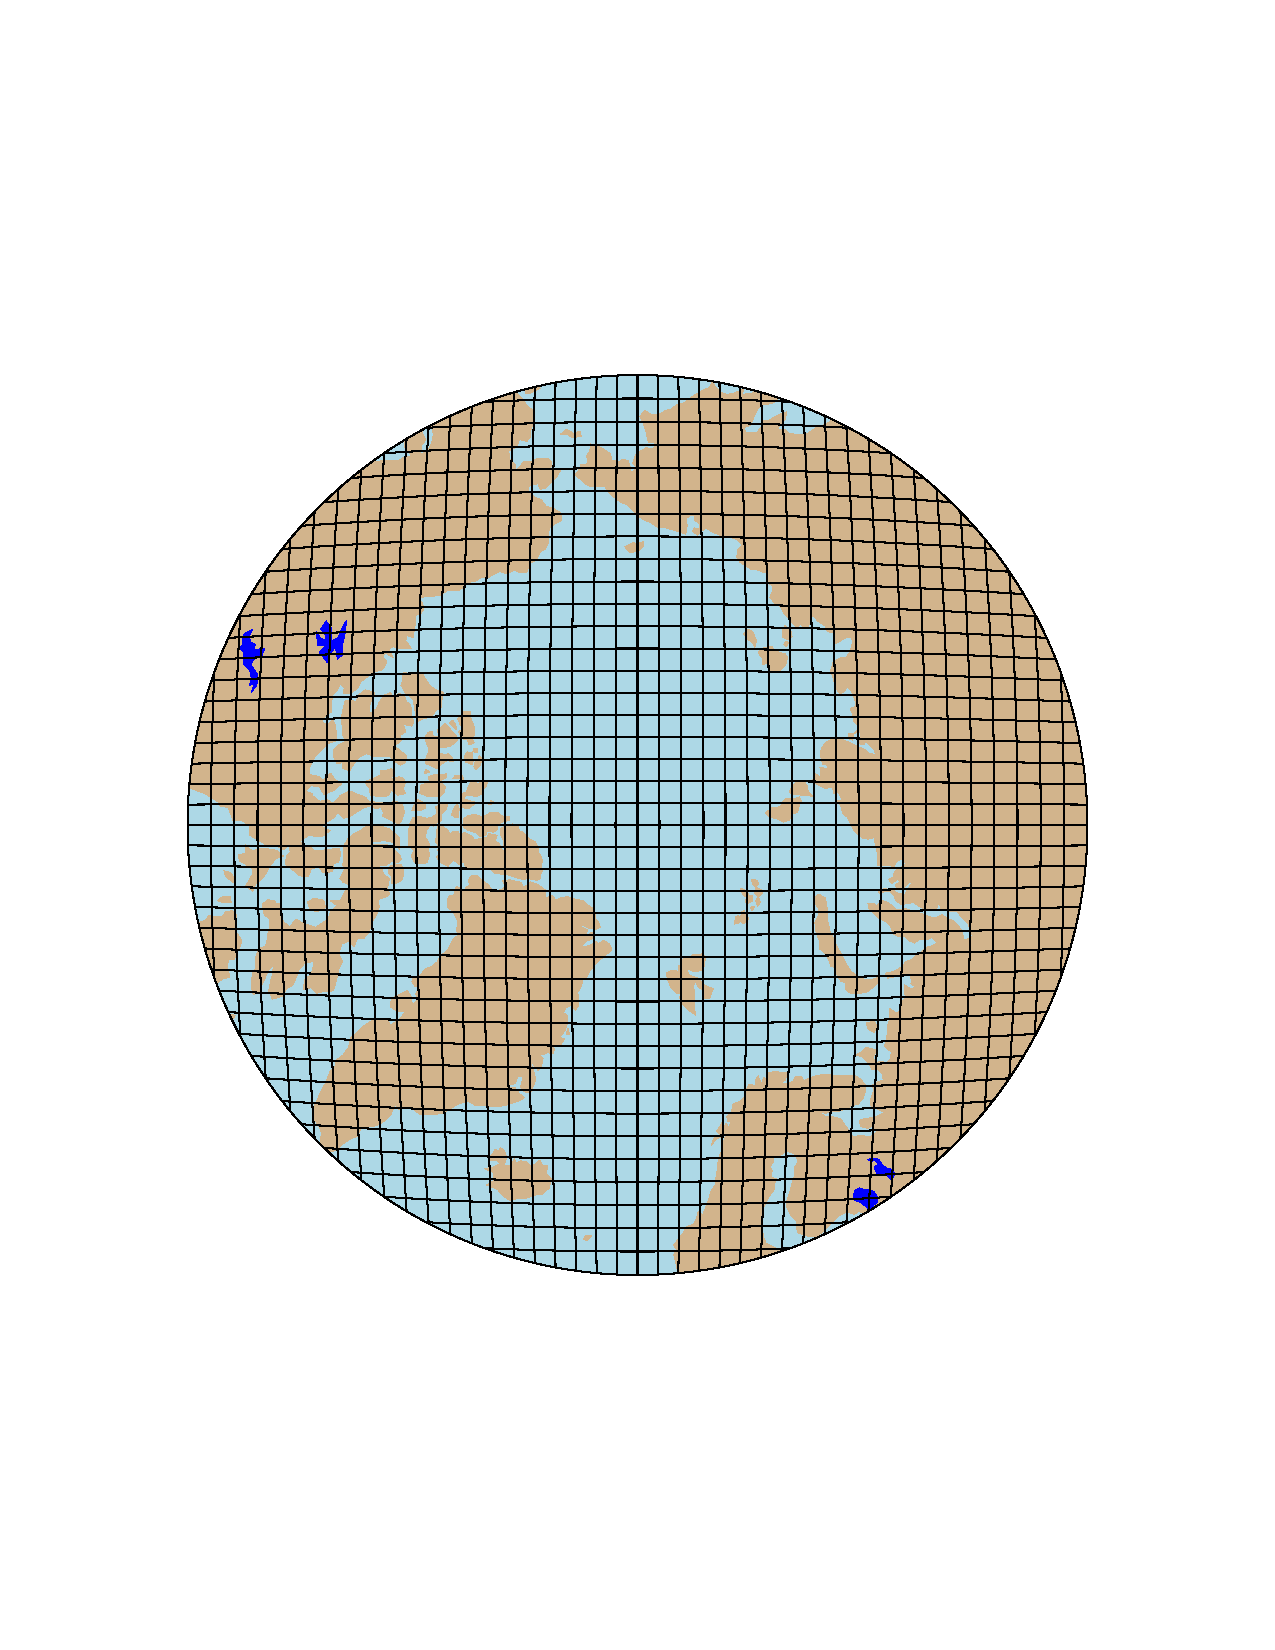
\includegraphics[width=60mm]{figs/grid-ne30pg2.pdf}&
         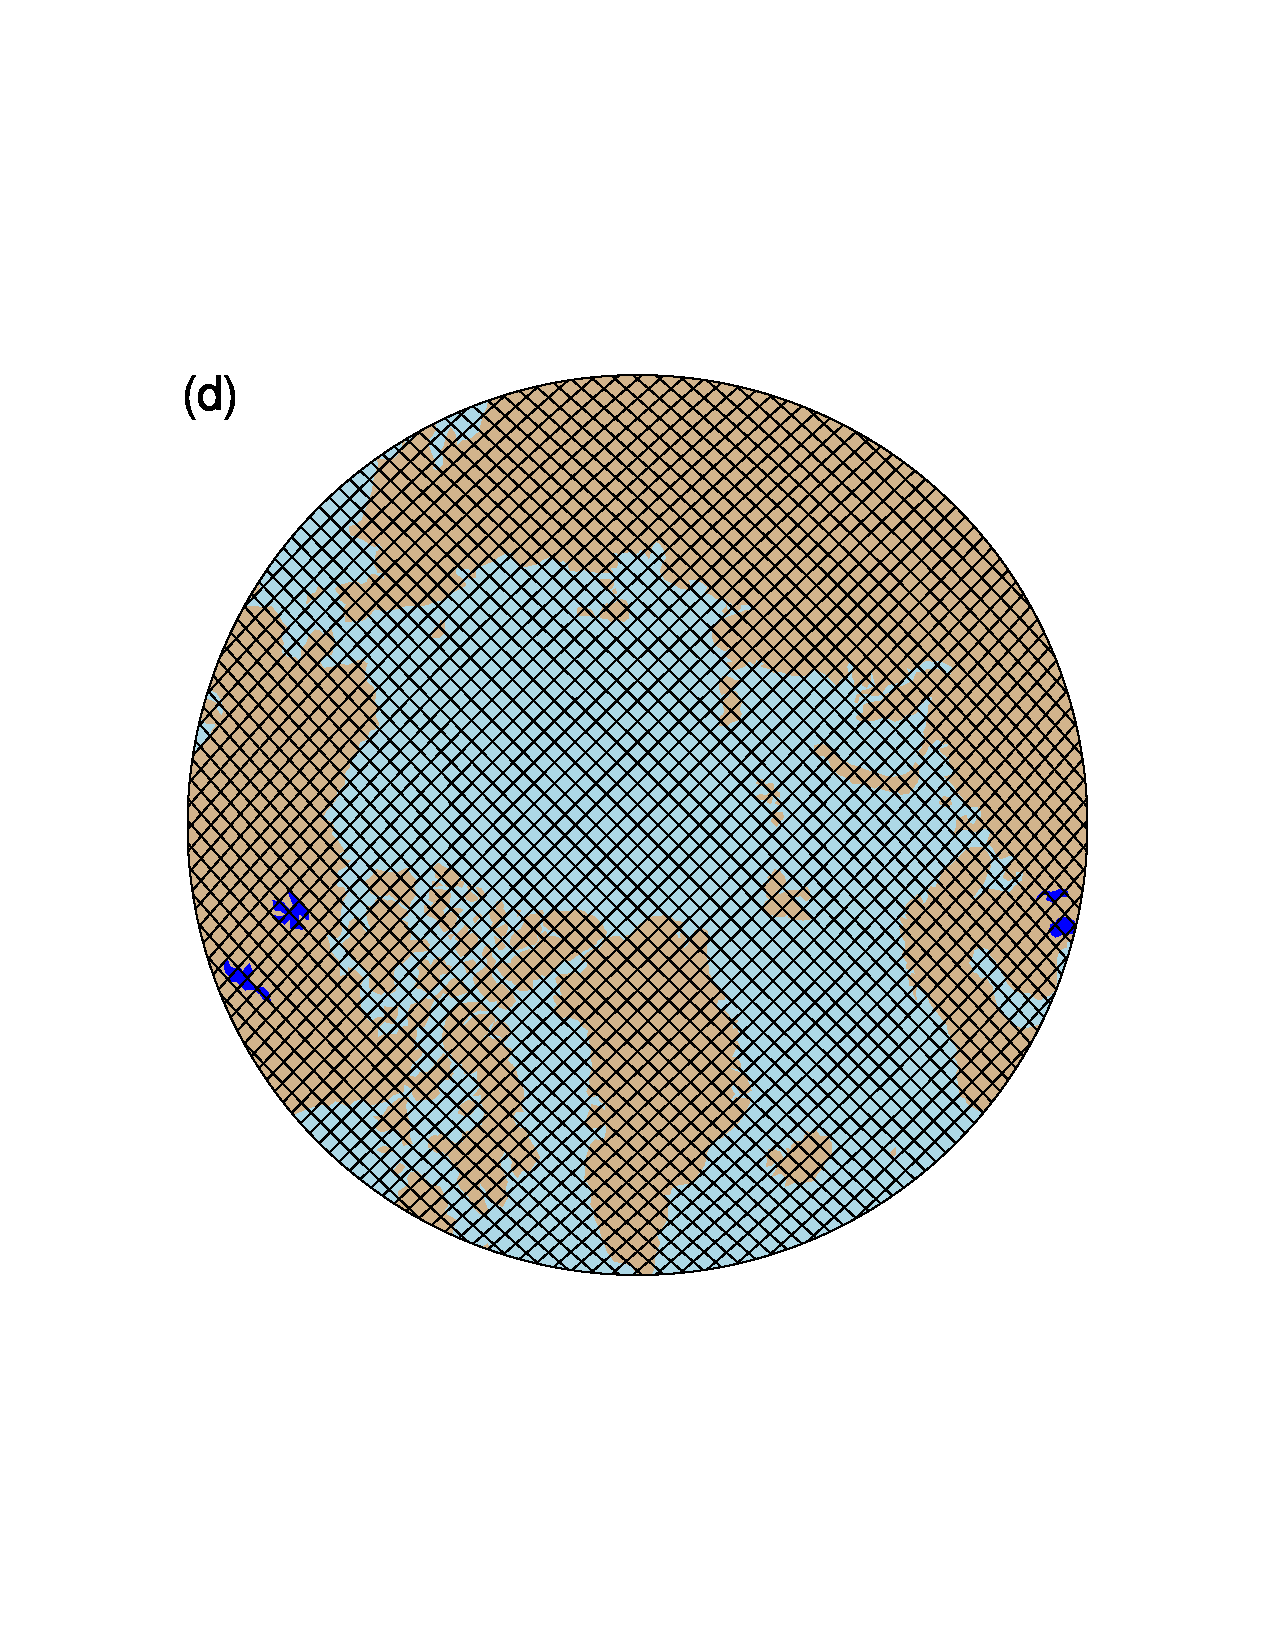
\includegraphics[width=60mm]{figs/grid-ne30pg3.pdf} \\
\end{tabular}
\end{center}
\caption{.}
\label{fig:uni-grids}
\end{figure}

\section{Methods}\label{sec:methods}
\subsection{Grids}
\subsection{Dynamical cores}
\subsubsection{Finite-volume model}
\subsubsection{Spectral-element model}
\subsection{Physical parameterizations}
\subsection{Experimental desing}
\subsection{Observational datasets}
\subsubsection{ERA5}
\subsubsection{LIVVkit 2.1}
\subsection{TempestExtremes}
\subsection{StormCompositer}

\section{Results}\label{sec:results}

\subsection{Tropospheric temperatures}
\subsection{Inter-annual variability}
\subsection{Synoptic-scale storm characteristics}
\subsection{Orographic gravity waves emanating from Greenland}
\subsection{Katabatic winds emanating from Greenland}
\subsection{Greenland surface mass balance}

% \section{Materials and Methods}
% Here is text on Materials and Methods.
%
% \subsection{A descriptive heading about methods}
% More about Methods.
%
% \section{Data} (Or section title might be a descriptive heading about data)
%
% \section{Results} (Or section title might be a descriptive heading about the
% results)
%

\section{Conclusions}\label{sec:conclusions}

\begin{figure}[t]
\begin{center}
         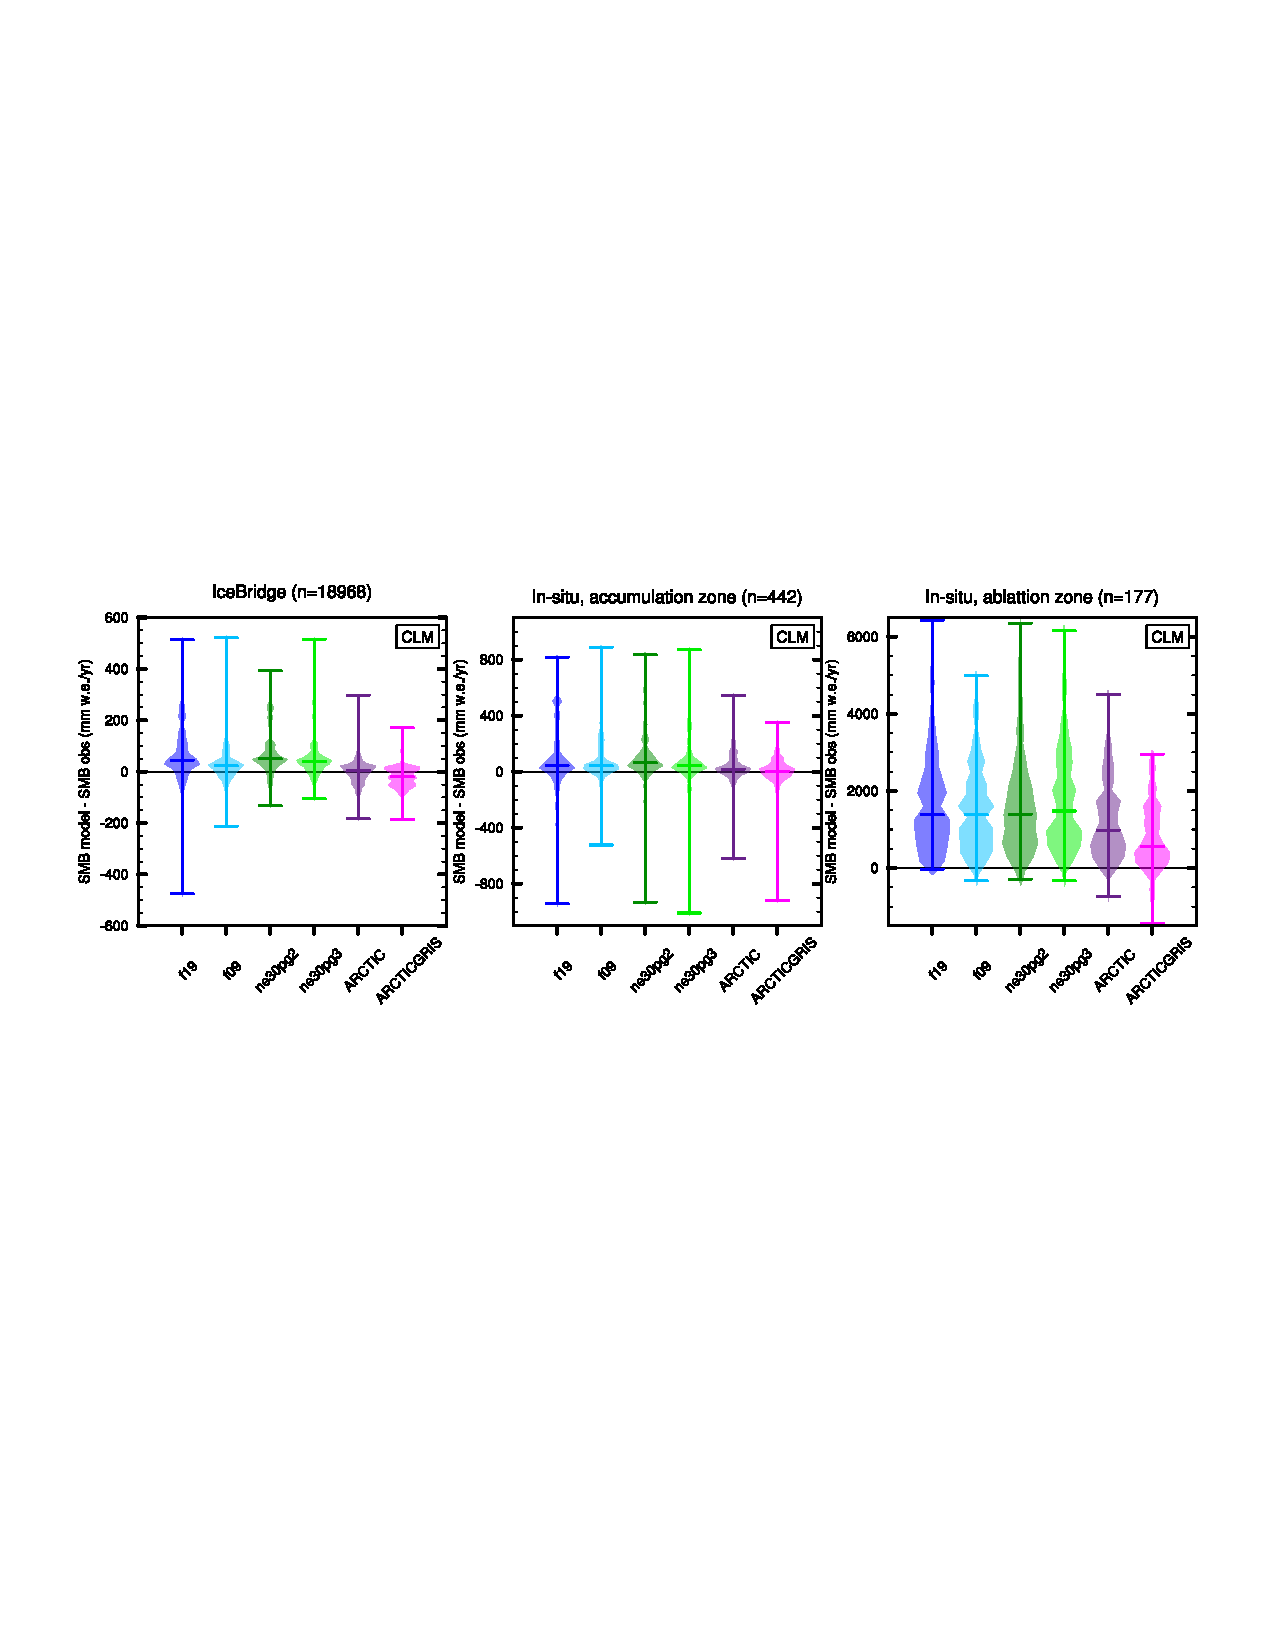
\includegraphics[width=130mm]{figs/temp_violens.pdf}
\end{center}
\caption{.}
\label{fig:pointdiff}
\end{figure}

\begin{figure}[t]
\begin{center}
         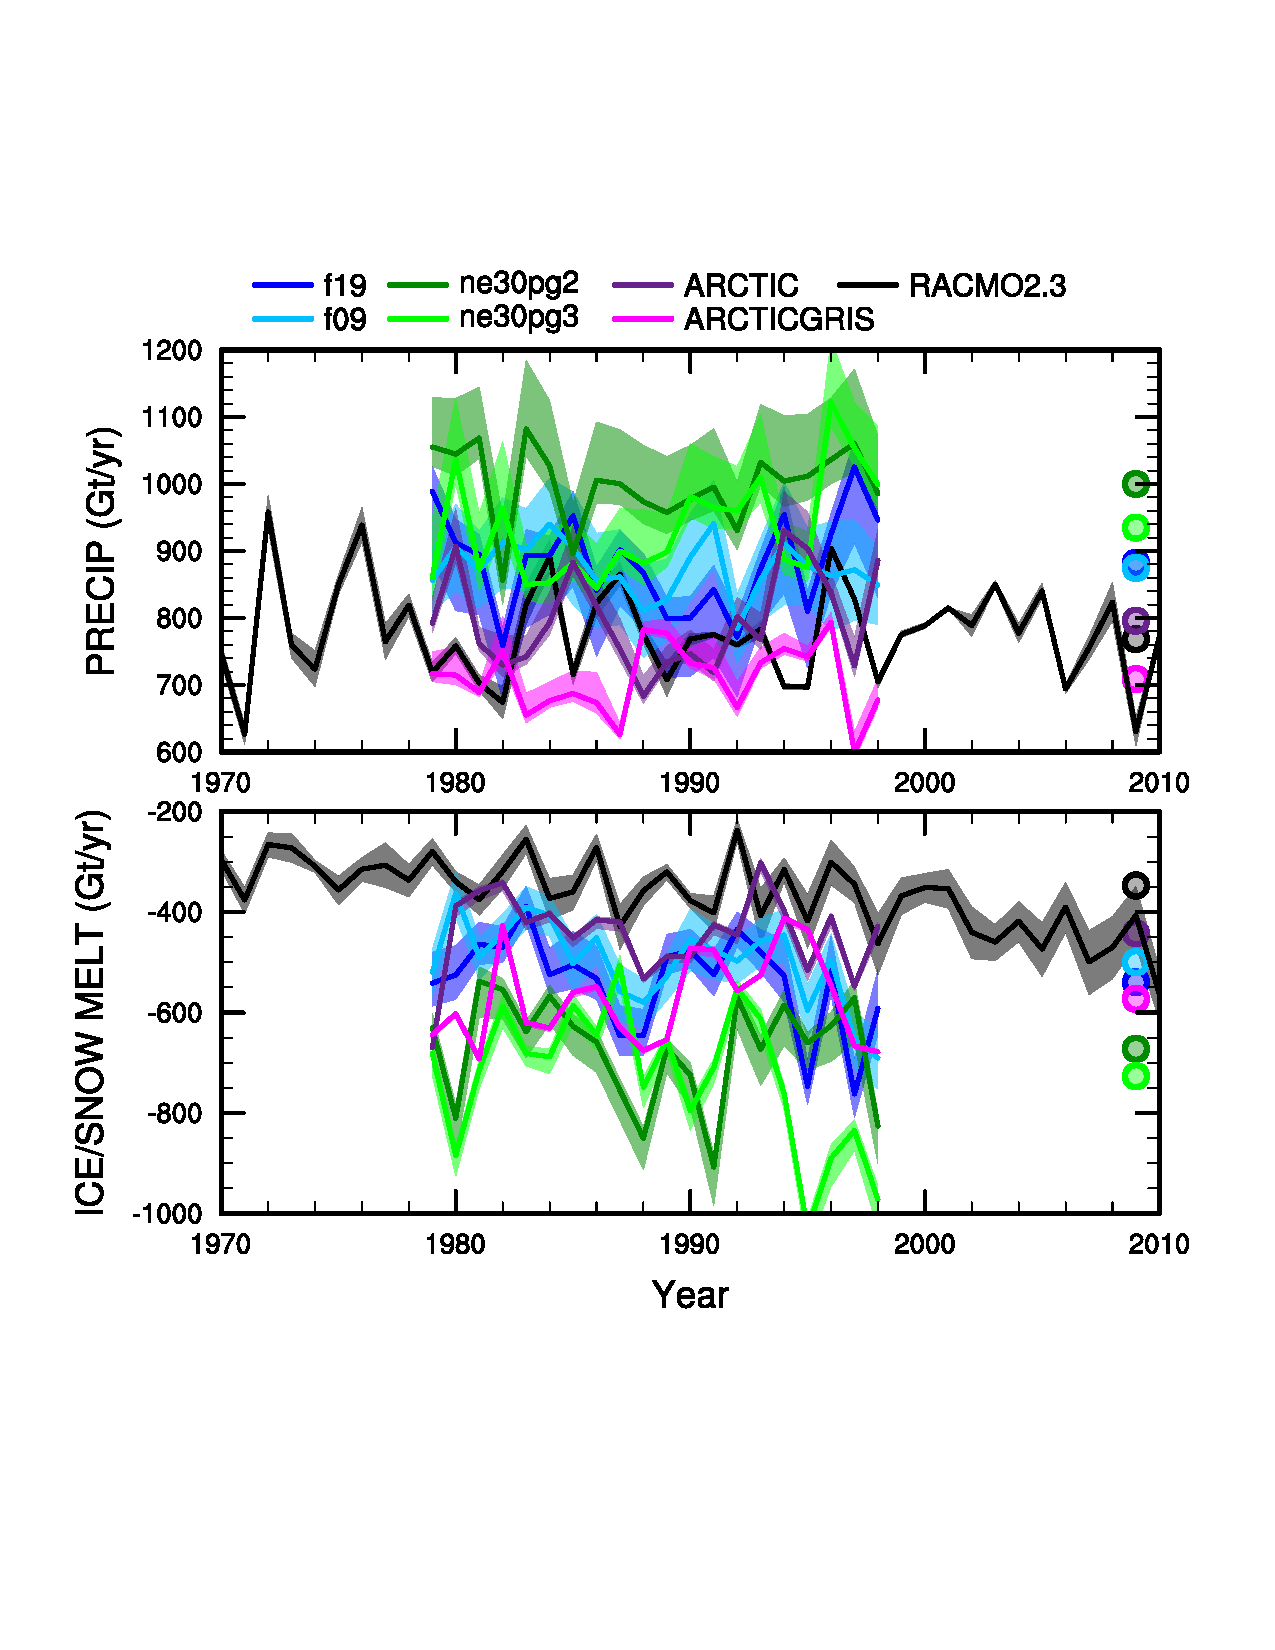
\includegraphics[width=100mm]{figs/temp_tseries_GRIS.pdf}
\end{center}
\caption{.}
\label{fig:tseries}
\end{figure}

\begin{figure}[t]
\begin{center}
         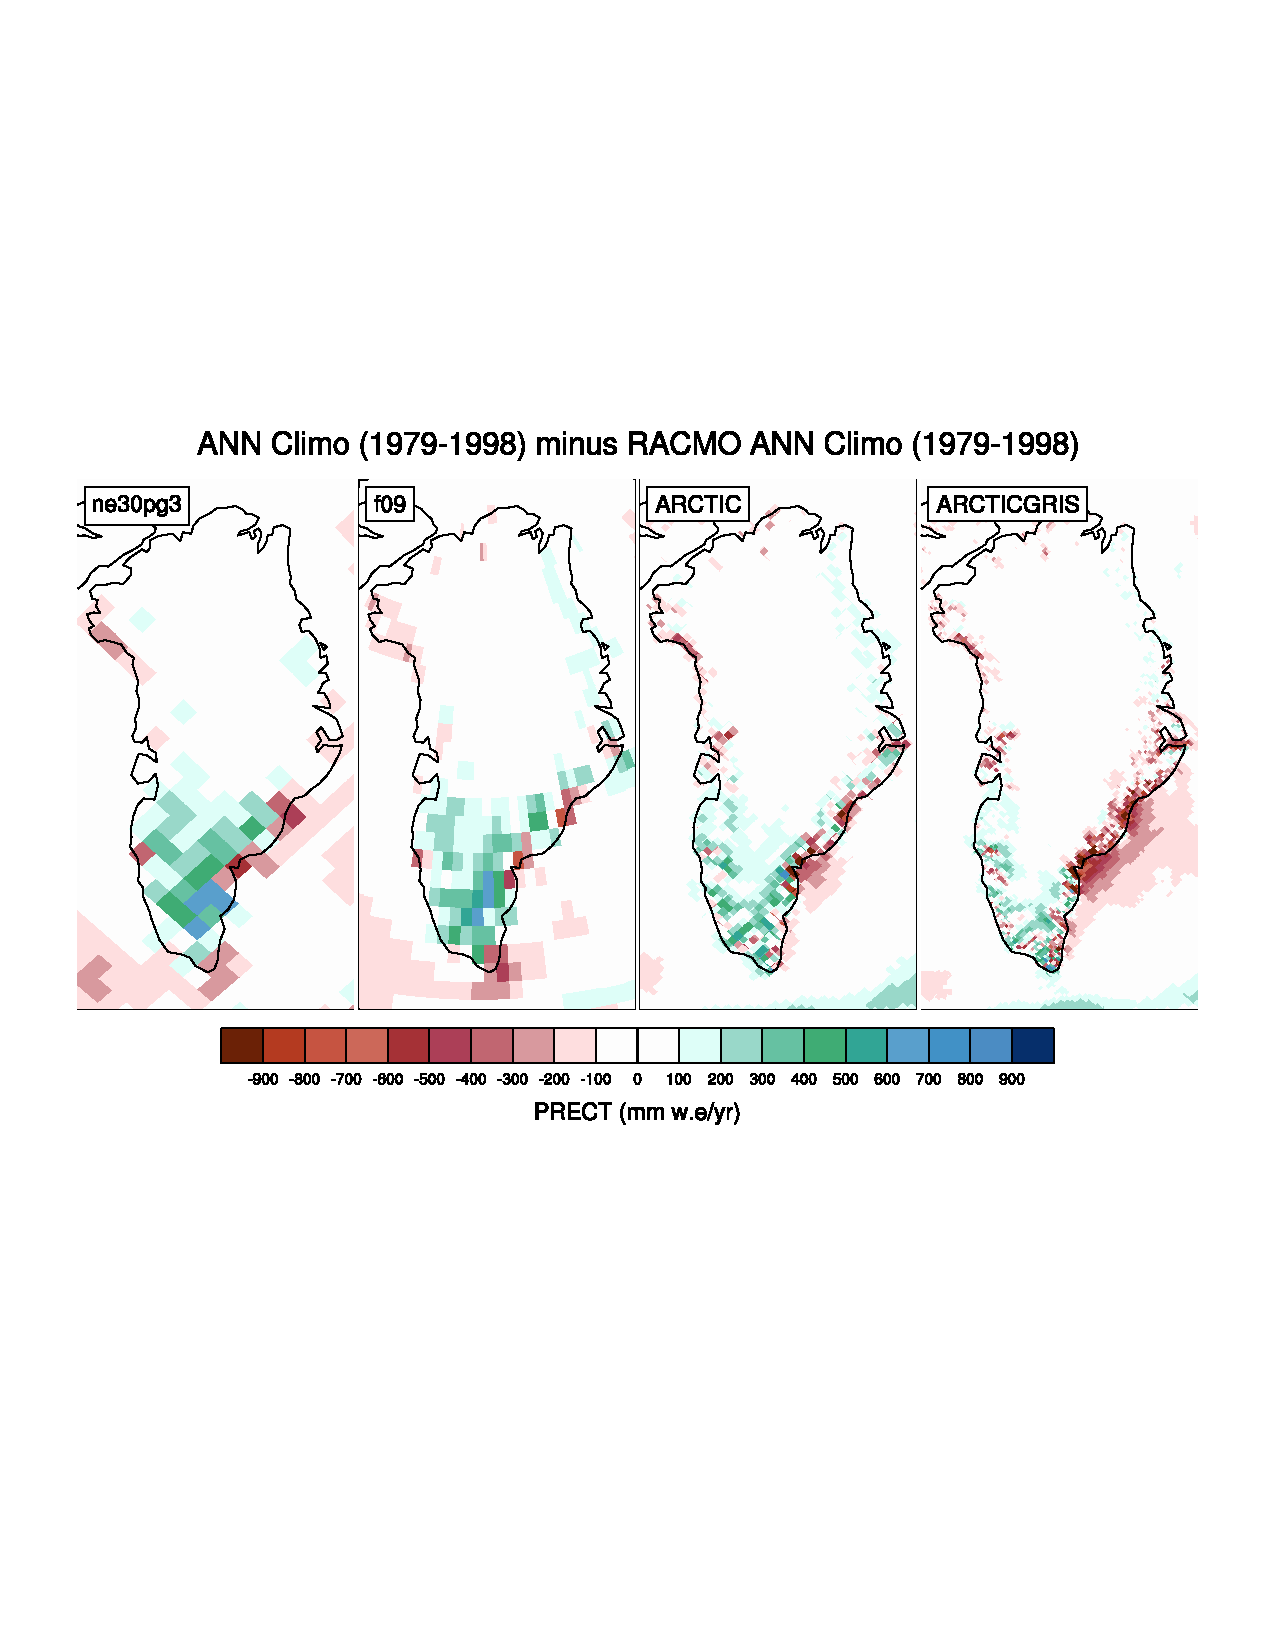
\includegraphics[width=130mm]{figs/temp_PRECT.pdf}
\end{center}
\caption{.}
\label{fig:prect}
\end{figure}

%Text here ===>>>


%%

%  Numbered lines in equations:
%  To add line numbers to lines in equations,
%  \begin{linenomath*}
%  \begin{equation}
%  \end{equation}
%  \end{linenomath*}



%% Enter Figures and Tables near as possible to where they are first mentioned:
%
% DO NOT USE \psfrag or \subfigure commands.
%
% Figure captions go below the figure.
% Table titles go above tables;  other caption information
%  should be placed in last line of the table, using
% \multicolumn2l{$^a$ This is a table note.}
%
%----------------
% EXAMPLE FIGURES
%
% \begin{figure}
% \includegraphics{example.png}
% \caption{caption}
% \end{figure}
%
% Giving latex a width will help it to scale the figure properly. A simple trick is to use \textwidth. Try this if large figures run off the side of the page.
% \begin{figure}
% \noindent\includegraphics[width=\textwidth]{anothersample.png}
%\caption{caption}
%\label{pngfiguresample}
%\end{figure}
%
%
% If you get an error about an unknown bounding box, try specifying the width and height of the figure with the natwidth and natheight options. This is common when trying to add a PDF figure without pdflatex.
% \begin{figure}
% \noindent\includegraphics[natwidth=800px,natheight=600px]{samplefigure.pdf}
%\caption{caption}
%\label{pdffiguresample}
%\end{figure}
%
%
% PDFLatex does not seem to be able to process EPS figures. You may want to try the epstopdf package.
%

%
% ---------------
% EXAMPLE TABLE
%
% \begin{table}
% \caption{Time of the Transition Between Phase 1 and Phase 2$^{a}$}
% \centering
% \begin{tabular}{l c}
% \hline
%  Run  & Time (min)  \\
% \hline
%   $l1$  & 260   \\
%   $l2$  & 300   \\
%   $l3$  & 340   \\
%   $h1$  & 270   \\
%   $h2$  & 250   \\
%   $h3$  & 380   \\
%   $r1$  & 370   \\
%   $r2$  & 390   \\
% \hline
% \multicolumn{2}{l}{$^{a}$Footnote text here.}
% \end{tabular}
% \end{table}

%% SIDEWAYS FIGURE and TABLE
% AGU prefers the use of {sidewaystable} over {landscapetable} as it causes fewer problems.
%
% \begin{sidewaysfigure}
% \includegraphics[width=20pc]{figsamp}
% \caption{caption here}
% \label{newfig}
% \end{sidewaysfigure}
%
%  \begin{sidewaystable}
%  \caption{Caption here}
% \label{tab:signif_gap_clos}
%  \begin{tabular}{ccc}
% one&two&three\\
% four&five&six
%  \end{tabular}
%  \end{sidewaystable}

%% If using numbered lines, please surround equations with \begin{linenomath*}...\end{linenomath*}
%\begin{linenomath*}
%\begin{equation}
%y|{f} \sim g(m, \sigma),
%\end{equation}
%\end{linenomath*}

%%% End of body of article

%%%%%%%%%%%%%%%%%%%%%%%%%%%%%%%%
%% Optional Appendix goes here
%
% The \appendix command resets counters and redefines section heads
%
% After typing \appendix
%
%\section{Here Is Appendix Title}
% will show
% A: Here Is Appendix Title
%
%\appendix
%\section{Here is a sample appendix}

%%%%%%%%%%%%%%%%%%%%%%%%%%%%%%%%%%%%%%%%%%%%%%%%%%%%%%%%%%%%%%%%
%
% Optional Glossary, Notation or Acronym section goes here:
%
%%%%%%%%%%%%%%
% Glossary is only allowed in Reviews of Geophysics
%  \begin{glossary}
%  \term{Term}
%   Term Definition here
%  \term{Term}
%   Term Definition here
%  \term{Term}
%   Term Definition here
%  \end{glossary}

%
%%%%%%%%%%%%%%
% Acronyms
%   \begin{acronyms}
%   \acro{Acronym}
%   Definition here
%   \acro{EMOS}
%   Ensemble model output statistics
%   \acro{ECMWF}
%   Centre for Medium-Range Weather Forecasts
%   \end{acronyms}

%
%%%%%%%%%%%%%%
% Notation
%   \begin{notation}
%   \notation{$a+b$} Notation Definition here
%   \notation{$e=mc^2$}
%   Equation in German-born physicist Albert Einstein's theory of special
%  relativity that showed that the increased relativistic mass ($m$) of a
%  body comes from the energy of motion of the body—that is, its kinetic
%  energy ($E$)—divided by the speed of light squared ($c^2$).
%   \end{notation}




%%%%%%%%%%%%%%%%%%%%%%%%%%%%%%%%%%%%%%%%%%%%%%%%%%%%%%%%%%%%%%%%
%
%  ACKNOWLEDGMENTS
%
% The acknowledgments must list:
%
% >>>>	A statement that indicates to the reader where the data
% 	supporting the conclusions can be obtained (for example, in the
% 	references, tables, supporting information, and other databases).
%
% 	All funding sources related to this work from all authors
%
% 	Any real or perceived financial conflicts of interests for any
%	author
%
% 	Other affiliations for any author that may be perceived as
% 	having a conflict of interest with respect to the results of this
% 	paper.
%
%
% It is also the appropriate place to thank colleagues and other contributors.
% AGU does not normally allow dedications.


\acknowledgments
This material is based upon work supported by the National Center for Atmospheric Research (NCAR), which is a major facility sponsored by the NSF under Cooperative Agreement 1852977. Computing and data storage resources, including the Cheyenne supercomputer
(doi:10.5065/D6RX99HX), were provided by the Computational and Information Systems Laboratory (CISL) at NCAR.

The data presented in this manuscript is available at {\url{https://github.com/adamrher/2020-arcticgrids}}.



%% ------------------------------------------------------------------------ %%
%% References and Citations

%%%%%%%%%%%%%%%%%%%%%%%%%%%%%%%%%%%%%%%%%%%%%%%
%
% \bibliography{<name of your .bib file>} don't specify the file extension
%
% don't specify bibliographystyle
%%%%%%%%%%%%%%%%%%%%%%%%%%%%%%%%%%%%%%%%%%%%%%%

%\bibliography{ enter your bibtex bibliography filename here }
\bibliography{bib}


%Reference citation instructions and examples:
%
% Please use ONLY \cite and \citeA for reference citations.
% \cite for parenthetical references
% ...as shown in recent studies (Simpson et al., 2019)
% \citeA for in-text citations
% ...Simpson et al. (2019) have shown...
%
%
%...as shown by \citeA{jskilby}.
%...as shown by \citeA{lewin76}, \citeA{carson86}, \citeA{bartoldy02}, and \citeA{rinaldi03}.
%...has been shown \cite{jskilbye}.
%...has been shown \cite{lewin76,carson86,bartoldy02,rinaldi03}.
%... \cite <i.e.>[]{lewin76,carson86,bartoldy02,rinaldi03}.
%...has been shown by \cite <e.g.,>[and others]{lewin76}.
%
% apacite uses < > for prenotes and [ ] for postnotes
% DO NOT use other cite commands (e.g., \citet, \citep, \citeyear, \nocite, \citealp, etc.).
%



\end{document}



More Information and Advice:

%% ------------------------------------------------------------------------ %%
%
%  SECTION HEADS
%
%% ------------------------------------------------------------------------ %%

% Capitalize the first letter of each word (except for
% prepositions, conjunctions, and articles that are
% three or fewer letters).

% AGU follows standard outline style; therefore, there cannot be a section 1 without
% a section 2, or a section 2.3.1 without a section 2.3.2.
% Please make sure your section numbers are balanced.
% ---------------
% Level 1 head
%
% Use the \section{} command to identify level 1 heads;
% type the appropriate head wording between the curly
% brackets, as shown below.
%
%An example:
%\section{Level 1 Head: Introduction}
%
% ---------------
% Level 2 head
%
% Use the \subsection{} command to identify level 2 heads.
%An example:
%\subsection{Level 2 Head}
%
% ---------------
% Level 3 head
%
% Use the \subsubsection{} command to identify level 3 heads
%An example:
%\subsubsection{Level 3 Head}
%
%---------------
% Level 4 head
%
% Use the \subsubsubsection{} command to identify level 3 heads
% An example:
%\subsubsubsection{Level 4 Head} An example.
%
%% ------------------------------------------------------------------------ %%
%
%  IN-TEXT LISTS
%
%% ------------------------------------------------------------------------ %%
%
% Do not use bulleted lists; enumerated lists are okay.
% \begin{enumerate}
% \item
% \item
% \item
% \end{enumerate}
%
%% ------------------------------------------------------------------------ %%
%
%  EQUATIONS
%
%% ------------------------------------------------------------------------ %%

% Single-line equations are centered.
% Equation arrays will appear left-aligned.

Math coded inside display math mode \[ ...\]
 will not be numbered, e.g.,:
 \[ x^2=y^2 + z^2\]

 Math coded inside \begin{equation} and \end{equation} will
 be automatically numbered, e.g.,:
 \begin{equation}
 x^2=y^2 + z^2
 \end{equation}


% To create multiline equations, use the
% \begin{eqnarray} and \end{eqnarray} environment
% as demonstrated below.
\begin{eqnarray}
  x_{1} & = & (x - x_{0}) \cos \Theta \nonumber \\
        && + (y - y_{0}) \sin \Theta  \nonumber \\
  y_{1} & = & -(x - x_{0}) \sin \Theta \nonumber \\
        && + (y - y_{0}) \cos \Theta.
\end{eqnarray}

%If you don't want an equation number, use the star form:
%\begin{eqnarray*}...\end{eqnarray*}

% Break each line at a sign of operation
% (+, -, etc.) if possible, with the sign of operation
% on the new line.

% Indent second and subsequent lines to align with
% the first character following the equal sign on the
% first line.

% Use an \hspace{} command to insert horizontal space
% into your equation if necessary. Place an appropriate
% unit of measure between the curly braces, e.g.
% \hspace{1in}; you may have to experiment to achieve
% the correct amount of space.


%% ------------------------------------------------------------------------ %%
%
%  EQUATION NUMBERING: COUNTER
%
%% ------------------------------------------------------------------------ %%

% You may change equation numbering by resetting
% the equation counter or by explicitly numbering
% an equation.

% To explicitly number an equation, type \eqnum{}
% (with the desired number between the brackets)
% after the \begin{equation} or \begin{eqnarray}
% command.  The \eqnum{} command will affect only
% the equation it appears with; LaTeX will number
% any equations appearing later in the manuscript
% according to the equation counter.
%

% If you have a multiline equation that needs only
% one equation number, use a \nonumber command in
% front of the double backslashes (\\) as shown in
% the multiline equation above.

% If you are using line numbers, remember to surround
% equations with \begin{linenomath*}...\end{linenomath*}

%  To add line numbers to lines in equations:
%  \begin{linenomath*}
%  \begin{equation}
%  \end{equation}
%  \end{linenomath*}



